\lecture{2}{Tue 21 Jan 2020 14:29}{Lab 2: Bode Plots}

\section{Introduction}
In this lab we learned about Bode plots and saw how their theoretical values corresponded with the real world outputs of our motor. 

\section{Deliverables}
\subsection{Bode Plots}
\begin{figure}[H]
	\centering
	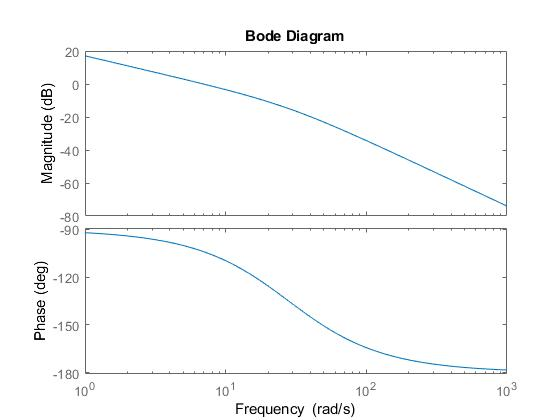
\includegraphics[width=0.8\textwidth]{./figures/lab2_theta.jpg}
	\caption{Bode plot for $\theta$ (Generated by MatLab)}
	\label{fig:}
\end{figure}

\begin{figure}[H]
	\centering
	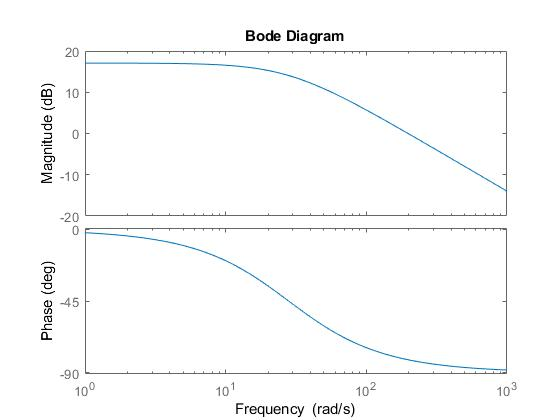
\includegraphics[width=0.8\textwidth]{./figures/lab2_omega.jpg}
	\caption{Bode plot for $\omega$ (Generated by MatLab)}
	\label{fig:}
\end{figure}

\subsection{Angular Position \& Velocity Plots}

\begin{figure}[H]
	\centering
	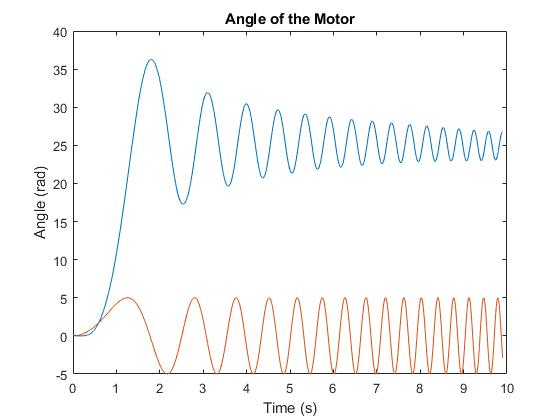
\includegraphics[width=0.8\textwidth]{./figures/lab2_theta_with_input.jpg}
	\caption{Motor Angular Position}
	\label{fig:}
\end{figure}

\begin{figure}[H]
	\centering
	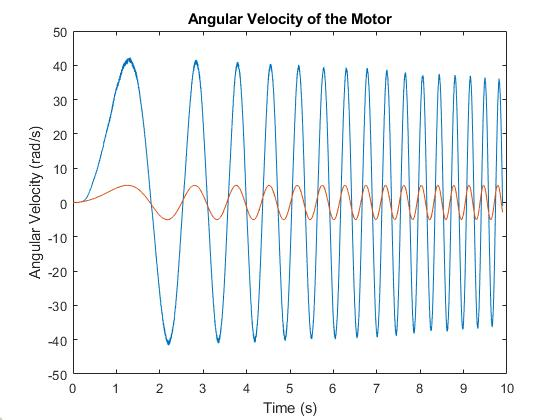
\includegraphics[width=0.8\textwidth]{./figures/lab2_omega_with_input.jpg}
	\caption{Motor Velocity}
	\label{fig:}
\end{figure}

For the plot of $\omega$, as the frequency increased, the amplitude stayed constant for a while and then began to slowly decrease, which matches the Bode plot. For the phase angle both sinusoids began at a phase angle of 0 degrees. As the frequency increased, the phase angle appears to decrease over time, but we could not quantify this difference because our test ended. 

For the plot of $\theta$, as frequency increased the amplitude decreased, which was predicted by the Bode plot. At very low frequencies, the amplitude tended towards very large values. The phase angle between the input and output signals can be seen to be $-90$ degrees, which agrees with our Bode plots.  

\subsection{Tabulated Data}

\begin{table}[H]
	\centering
	\caption{Data Collection Table}
	\label{tab:data-collection}
	\begin{tabular}{|| c c c c c c ||}
		\hline
		$\omega$ & Magnitude & Gain (dB) & Zero-Time Difference & Phase (rad) & Phase (deg) \\ [0.5ex]
		\hline\hline
		0.5 & 7.2805 & 17.2433 & 0.2364 & 0.1182 & -6.7726 \\
		\hline
		0.7896 & 6.9883 & 16.8875 & 0.0467 & 0.0368 & -2.1106 \\
		\hline 
		1.2469 & 7.037 & 16.3012 & -0.0597 & 0.0745 & 4.2661 \\
		\hline 
		1.9692 & 7.2075 & 17.1557 & 0.0183 & 0.0361 & -2.0663 \\
		\hline
		3.1098 & 6.9883 & 16.8875 & 0.0509 & 0.1582 & -9.0661 \\
		\hline
		4.911 & 6.8666 & 16.7348 & -0.0079 & -0.00386 & 2.2102 \\
		\hline 
		7.7554 & 6.5501 & 16.3249 & 0.0295 & 0.2285 & -13.0901 \\
		\hline 
		12.2474 & 5.99 & 15.5486 & 0.0317 & 0.3888 & -22.2763 \\
		\hline 
		19.3413 & 5.3813 & 14.6177 & 0.0268 & 0.5181 & -29.6827 \\
		\hline 
		30.5439 & 4.6751 & 13.3959 & 0.00206 & 0.6284 & -36.0026 \\
		\hline 
		48.2352 & 3.0924 & 9.8059 & 0.0174 & 0.841 & -48.1836 \\
		\hline 
		76.1734 & 3.0924 & 9.8059 & 0.0114 & 0.8668 & -49.6612 \\
		\hline 
		120.2936 & 2.3132 & 7.2843 & 0.0089 & 1.0757 & -61.6309 \\
		\hline 
		189.9696 & 1.7288 & 4.755 & 0.0077 & 1.4687 & -84.1504 \\
		\hline 
		300 & 1.534 & 3.7167 & 0.0068 & 2.0292 & -116.2648 \\
		\hline 
	\end{tabular}
\end{table}

\subsection{Experimental Bode Plots}

\begin{figure}[H]
	\centering
	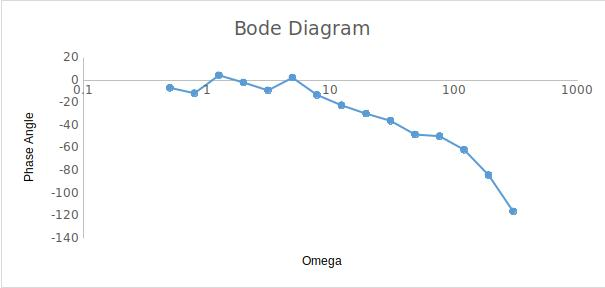
\includegraphics[width=0.8\textwidth]{./figures/lab2_experiment_phase.jpg}
	\caption{Experimental Bode Plot for the Phase Angle of $\theta$}
	\label{fig:}
\end{figure}

\begin{figure}[H]
	\centering
	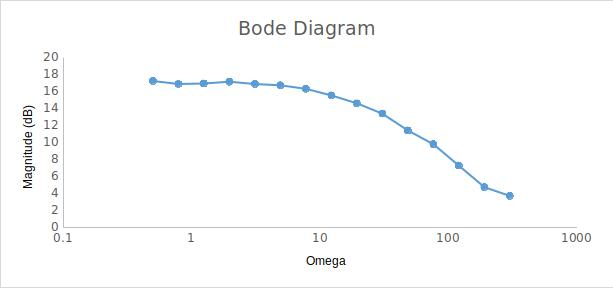
\includegraphics[width=0.8\textwidth]{./figures/lab2_experiment_magnitude.jpg}
	\caption{Experimental Bode Plot for Phase Amplitude of $\theta$}
	\label{fig:}
\end{figure}

Our experimental bode plot for the amplitude of $\theta$ resembles the shape of the one plotted in MatLab, despite some variance in the individual points. Our plot for the phase angle of $\theta$ is much more varied. We received very different results running the experiment with high frequencies due to measurement error. (Each peak was only recorded as a single data point.) Thus our Bode plot for $\theta$ doesn't resemble the calculated one as closely.
